\thispagestyle{empty}
\begin{center}
    \vspace*{3cm}\alt\bfseries\fortypt Introduzione\\[15pt]
    \raisebox{15pt}{\scalebox{.6}{\pgfornament{88}}}
\end{center}
%
% Introduction
%
Ottimizzare significa trovare la soluzione migliore per un problema,
nell'insieme delle sue soluzioni ammissibili. La necessità di risolvere un
problema all'ottimo è così comune che il concetto di ottimizzazione è ormai
parte di ogni ambito che richieda di risolvere problemi decisionali.
L'obiettivo è quello di ottimizzare una grandezza assegnando dei valori
alle variabili da cui dipende e rispettando un insieme di vincoli che
limitano i valori ammissibili per queste variabili.  Nell'ottica di
impiegare modelli matematici per risolvere problemi decisionali, spesso è
possibile esprimere la grandezza da ottimizzare come una funzione da
minimizzare o massimizzare. Allo stesso modo, i vincoli del problema
possono essere modellati con delle funzioni che assumono un insieme
limitato di valori.

La ricerca operativa è un ramo della matematica applicata che si occupa di
risolvere problemi decisionali impiegando metodi e modelli matematici.
La sfida principale di fronte a un problema reale è la ricerca di un modello
che sia in grado di descriverlo adeguatamente. A questo riguardo, la
formulazione di un modello dovrebbe essere sufficientemente complessa da
riflettere fedelmente il problema cui si riferisce e, allo stesso tempo,
abbastanza semplice da renderlo trattabile con gli strumenti risolutivi
disponibili. La soluzione di un modello matematico viene poi analizzata e
interpretata per studiarne l'effettiva applicabilità, in relazione al
problema reale. Il processo di modellazione e risoluzione può anche essere
iterato, con la finalità di perfezionare il modello e ottenere soluzioni
più accurate.

\begin{figure}[h]
    \centering
    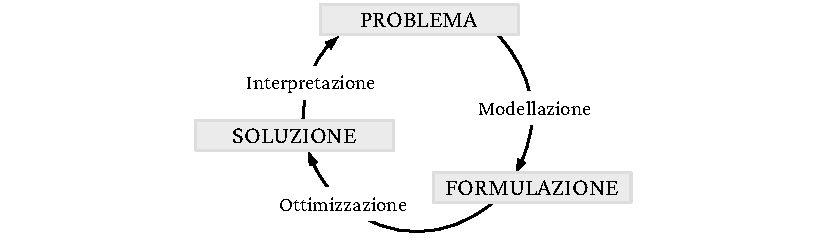
\includegraphics[scale=1]{INTRO_opt-cycle}
    \caption*{Figura: Processo di ottimizzazione \cite{GITO}.}
    \label{fig:INTRO_opt-cycle}
\end{figure}

